\section{Online Computation}
Offline computation is carried out once and the dependency files are saved. Every time the video is played, the online computation loads the dependency files, computes a selective mask for each frame and decodes according to the mask.

\subsection{Selective Mask Computation}
Selective mask indicates the macroblocks that the decoder needs to decode as '1' and the rest as '0'. It considers both inter-frame and intra-frame dependencies. Note that the inter-frame dependency has to be computed first. If intra-frame dependency is computed first, when computing inter-frame dependency, the computation will select some new P-macroblocks and I-macroblocks. Since the intra-frame dependency for the newly selected I-macroblocks is not computed, this leads to decoding errors at those I-macroblocks. The error will subsequently affect the motion compensation decoding at other macroblocks using those I-macroblocks as reference. By contrast, if inter-frame dependency is computed first, the intra-frame computation will select only I-macroblocks because DC\&AC prediction coding only applies to I-macroblock. Since inter-frame dependency does not apply to I-macroblocks, the newly selected I-macroblocks won't introduce errors. 

\subsubsection{Inter-frame Dependency Computation}
Inter-frame dependency is caused by motion compensation decoding. A MPEG4 SP GOP consists of an I frame followed by a sequence of P frames. The P-macroblocks of every P frame are motion compensated with reference to macroblocks of its previous frame. This means every P frame is dependent on its previous frame. Therefore we compute the inter-frame dependency from last frame back to the first frame of the GOP. The dependencies are shown as Fig 5(a).
 
\begin{figure}
%\vspace{2.5cm}
\centering
%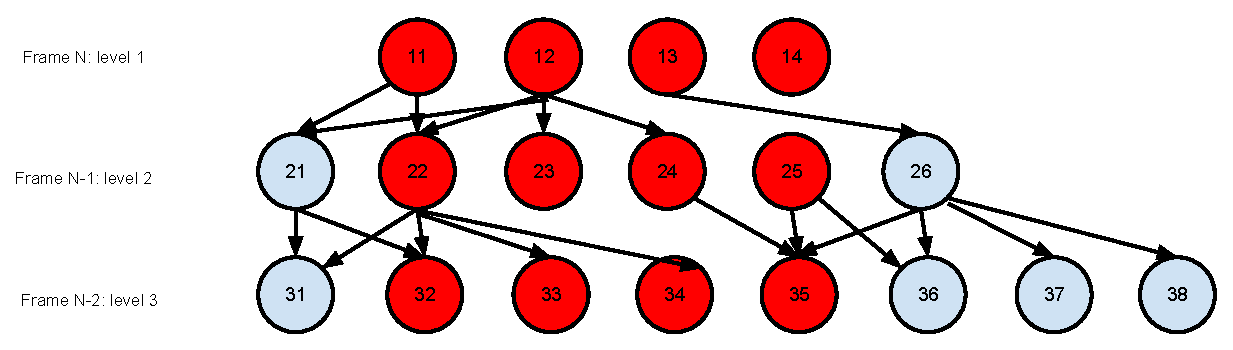
\includegraphics[height=2.5cm]{inter.eps}
\subfigure[Inter-frame Graph]{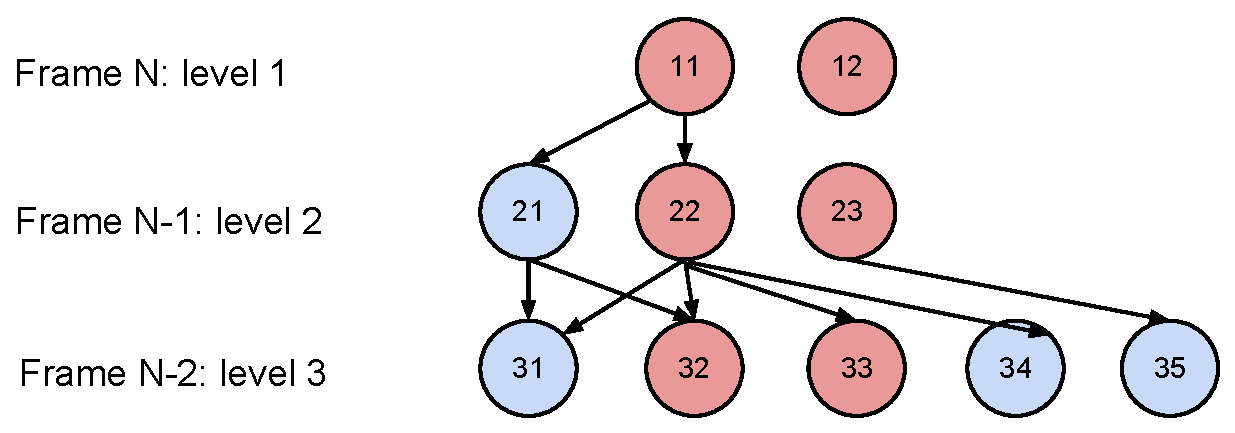
\includegraphics[height=1.6cm]{interc1.eps}}
\quad\quad
\subfigure[Modified Inter-frame Graph]{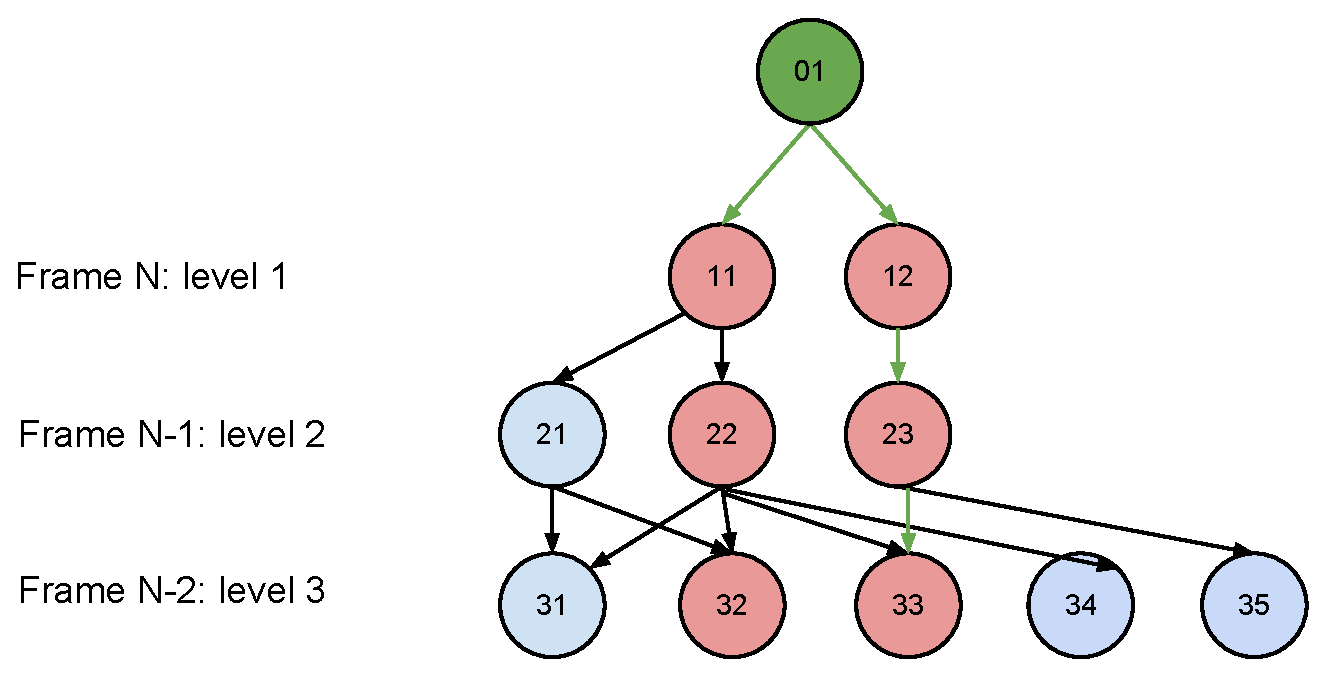
\includegraphics[height=2.5cm]{interc2.eps}}
\caption{Inter-frame Dependency Abstraction} 
\end{figure}
Suppose frame N is the last frame of the GOP, the figure shows the dependencies in three frames. The macroblocks and the dependencies form a graph. By adding a pseudo root node and edges connecting the ROI macroblocks, the graph is transformed to a weakly connected directed acyclic graph shown as Fig 5(b). With this modification, the graph traversal algorithm Depth-First Traversal (DFT) or Breadth-First Traversal (BFT) can be applied. The macroblocks that are visited by the graph traversal are selected, while the rest are not needed. 

\subsubsection{Intra-frame Dependency Computation} 
Similar to Inter-frame dependency, Intra-frame dependency computation can be abstracted to graph traversal problems. 

\begin{figure}
%\vspace{2.5cm}
\centering
\subfigure[Graph]{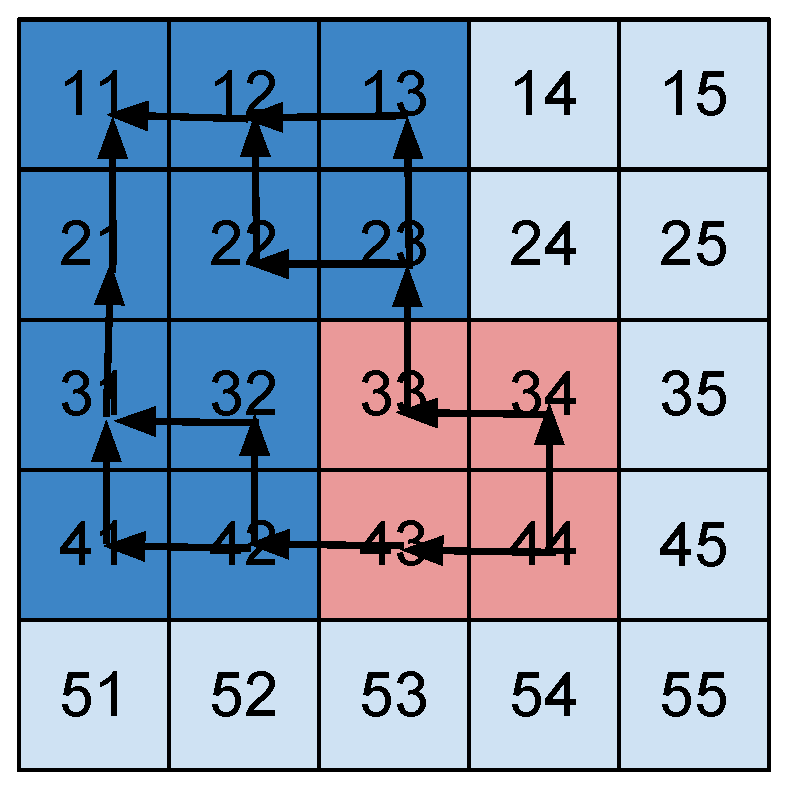
\includegraphics[height=2.2cm]{intrac3.eps}}
\quad\quad\quad
\subfigure[Optimization]{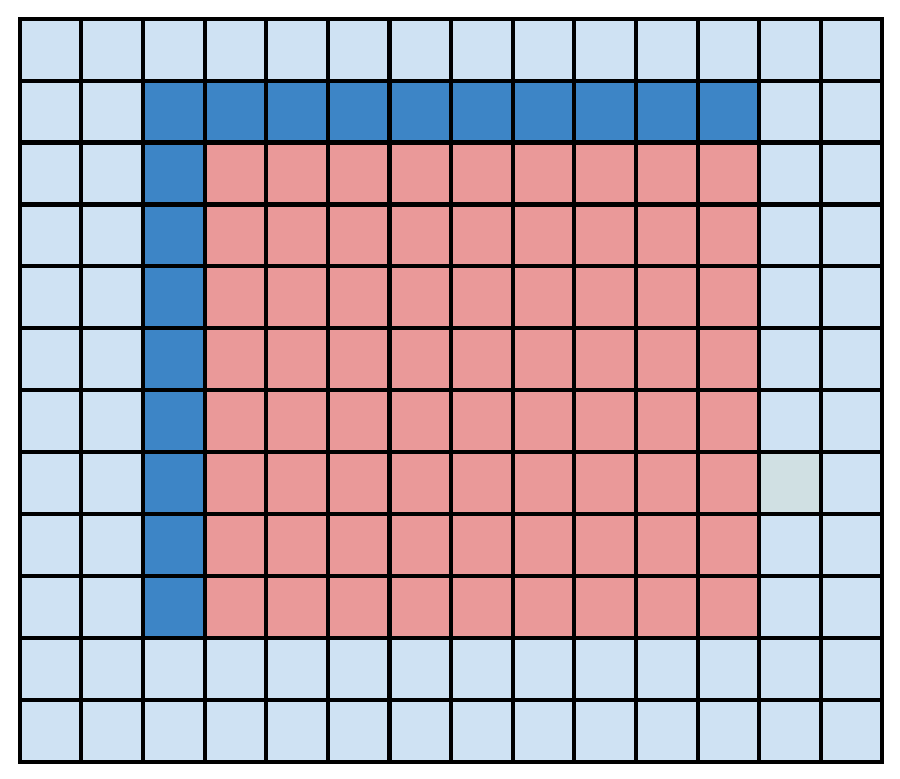
\includegraphics[height=2.2cm]{intrac2.eps}}
%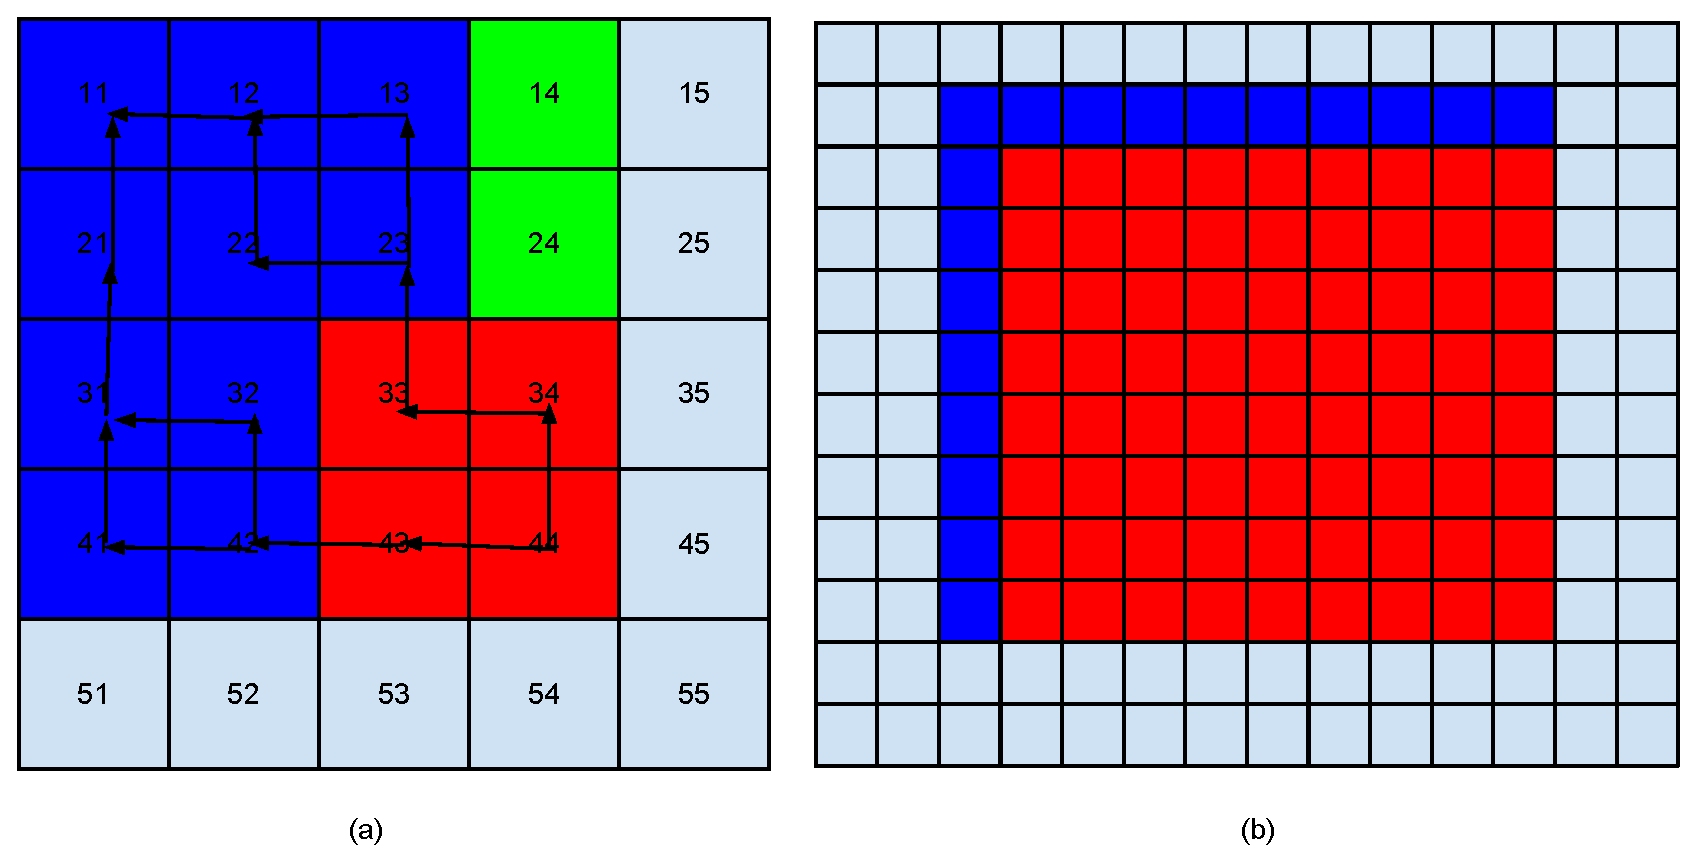
\includegraphics[height=2.5cm]{intra.eps}
\caption[intra.eps]{Intra-frame Dependency and the Optimization}
\end{figure}
In Fig 7(a), macroblock 33, 34, 43 and 44 are ROI macroblocks. The dependency graph due to DC\&AC prediction coding is depicted. Because the dependency direction is always pointing up or left, the graph rooted at a macroblock is always formed by one of the graphs rooted at the first row and first column macroblocks of the ROI and some macroblocks within the ROI. Therefore, an optimization is to apply graph traversal algorithms only on the macroblocks at upper and left edges of the ROI, and select all macroblocks within ROI. This is illustrated as Fig 7(b).

\subsection{Select the Bits}
In order to decode selectively, a mechanism is needed for the decoder to select the bits for selected macroblocks. Two approaches can be used to select the bits, namely bitstream reconstruction and bit seeking. In bitstream reconstruction, a new video bitstream is constructed according to the selective masks and the macroblock start and end positions. The newly constructed bitstream consists of only the macroblocks selected in selective masks. At bit seeking approach, we instruct the decoder to seek to the start position of next selected macroblock at decoding. The second approach avoids the additional memory allocation for the new bitstream therefore it is the preferred approach in our research. However, for applications in the next streaming context, the first approach may provide better bandwidth utilization as the shorter reconstructed bitstream can be transmitted. 

%\subsection{Modifications of Decoder}
%The online computation requires modification for both motion decoding and texture decoding of standard MPEG4 SP decoder. For motion decoding, the MV values are loaded directly from MV dependency file. No MV prediction decoding is carried out. For texture decoding, the DC\&AC prediction direction is read from DC\&AC prediction direction file. mechanism of bits seeking is also added for the decoder to decode selectively. 
  

